\documentclass[border=0.2cm]{standalone}
 
\usepackage{tikz}
\usetikzlibrary{trees}
 
\begin{document}

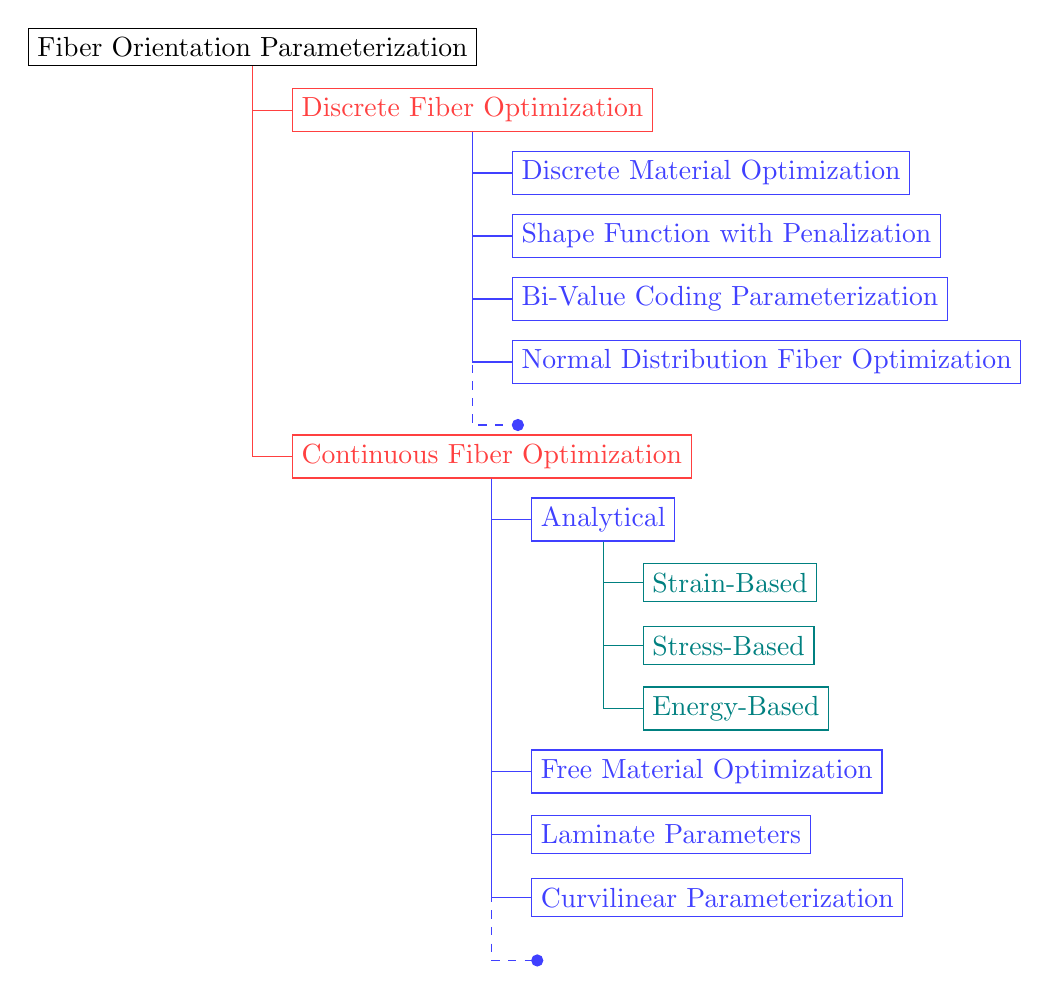
\begin{tikzpicture}
    [
        level 1/.style = {red!75},
        level 2/.style = {blue!75},
        level 3/.style = {teal},
        every node/.append style = {draw, anchor = west},
        grow via three points={one child at (0.5,-0.8) and two children at (0.5,-0.8) and (0.5,-1.6)},
        edge from parent path={(\tikzparentnode\tikzparentanchor) |- (\tikzchildnode\tikzchildanchor)}]
    
    \node {Fiber Orientation Parameterization}
    child {node {Discrete Fiber Optimization}
            child {node {Discrete Material Optimization}}
            child {node {Shape Function with Penalization}}
            child {node {Bi-Value Coding Parameterization}}
            child {node {Normal Distribution Fiber Optimization}}
            child {node [circle, fill, minimum size = 4pt, inner sep = 0] {} edge from parent [dashed] }
            edge from parent node [draw = none, left] {};
            % child {node [circle, fill, minimum size = 4pt, inner sep = 0] {}}
            % edge from parent [dashed]
        }
    child [missing] {}
    child [missing] {}
    child {node at (0, -2) {Continuous Fiber Optimization}
            child {node {Analytical}
                    child {node {Strain-Based }}
                    child {node {Stress-Based}}
                    child {node {Energy-Based}}}
            child [missing] {}
            child {node at (0, -1.6) {Free Material Optimization}}
            child {node at (0, -1.6) {Laminate Parameters}}
            child {node at (0, -1.6) {Curvilinear Parameterization}}
            child {node at (0, -1.6) [circle, fill, minimum size = 4pt, inner sep = 0] {} edge from parent [dashed]}
            edge from parent node [draw = none, left] {}};
    
\end{tikzpicture}

\end{document}